\documentclass[]{article}
\usepackage{amsmath}
\usepackage{amssymb}
\usepackage{amsthm}
\usepackage{listings}
\usepackage{multirow}
\usepackage{tikz}
\usepackage{tikz-qtree}
\usepackage{tipa}
\usetikzlibrary{arrows,automata}
\begin{document}

\title{COMS W3261 \\ Computer Science Theory \\ Lecture 3\\ Regular Expressions}
\author{Alexander Roth}
\date{2014-09-08}
\maketitle

\section*{Outline}
  \begin{itemize}
    \item Review
    \item Regular Expressions
    \item Examples of regular expressions
    \item Finite automata with epsilon transitions
  \end{itemize}

\section{Review}
  \begin{itemize}
    \item A deterministic finite automaton defines a regular language.
    \item In the last lecture we showed that using the subset construction we
          can transform a nondeterministic finite automaton into an equivalent
          DFA. Hence, NFA's also define the regular languages.
    \item An $\epsilon$-NFA is an NFA with epsilon transitions. Using the subset
          construction we can transform an $\epsilon$-NFA into an equivalent
          DFA. Hence, $\epsilon$-NFA's are also another way to define the
          regular languages.
    \item In this lecture we will define another very different formalism called
          regular expressions that provide yet another way to define the regular
          languages
  \end{itemize}

\section{Regular Expressions}
  \begin{itemize}
    \item A regular expression $E$ is an algebraic expression that denotes a
          language $L(E)$.
    \item Programming languages such as awk, java, javascript, perl, python use
          regular expressions to match patterns in strings.
    \item There are differences in the regular expression notations used by
          various programming languages, the most common variants being POSIX
          regular expressions and perl-compatible regular expressions.
    \item Virtually all regular-expressions notations have the operations of
          union, concatenation, and Kleene closure. We shall call regular
          expressions with just these three operator Kleene regular expressions.
  \end{itemize}

  \subsection*{Kleene regular expressions}
    \begin{itemize}
      \item We can specify Kleene regular expressions over an alphabet $\Sigma$
            and the languages they denote using the following inductive
            definition:
        \begin{itemize}
          \item The constants \textepsilon \, and $\phi$ are regular
                expressions that denote the language \{ \textepsilon \, \} and
                \{ \, \}, respectively.
          \item A symbol $c$ in $\Sigma$ by itself is a regular expression that
                denotes the language \{ $c$ \}
        \end{itemize}
      \item Induction: Let $E$ and $F$ be regular expressions.
        \begin{itemize}
          \item $E + F$ is a regular expression that denotes $L(E) \cup L(F)$.
          \item $EF$ is a regular expression that denotes $L(E)L(F)$, the
                concatenation of $L(E)$ and $L(F)$.
          \item $E^*$ is a regular expression that denotes $(L(E))^*$.
          \item $(E)$ is a regular expression that denotes $L(E)$.
        \end{itemize}
      \item Precedence and associativity of the regular-expression operators
        \begin{itemize}
          \item The regular-expression operator star has the highest precedence
                and is left associative.
          \item The regular-expression operator concatenation has the next
                highest precedence and is left associative.
          \item The regular-expression operator $+$ has the lowest precedence
                and is left associative.
          \item Thus the regular expression $a + b * c$ would be grouped $a + ((
                b^*)c$.
        \end{itemize}
      \item If a regular expression $E$ denotes a language $L$ and a string $w$
            is in $L$, we will often say that $E$ \emph{matches} $w$.
    \end{itemize}

    \subsubsection*{Notes From Class}
      $a + b + c \equiv (a + b) + c$                   \\
      Let's look at a syntax tree for this expression: \\
        \Tree [.+ [.a ] [.concat [.b ] [.* c ] ] ]     \\
      $E = a + bc^*$ and the language is $L(E) =
      \{a, b, bc, bcc, bccc, \ldots \}$ \\
      $\{a\} \cup \{bc^i \, | \, i \geq 0 \} = \{ a, bc^i | i \geq 0 \}$ \\
      $E = a^*b^* \implies L(E) = \{ \epsilon, a, b, aa, ab, bb, \ldots \}$

  \subsection*{Examples of Kleene regular expressions and the languages they
  denote}
    \begin{itemize}
      \item $0^*10^*$ denotes the set of all strings of 0's and 1's containing a
            single 1.
      \item $(0 + 1)^*1(0 + 1)^*$ denotes the set of all strings of 0's and 1's
            containing at least one 1.
      \item $1^*(01^*01^*)^*$ denotes the set of all strings of 0's and 1's
            containing an even number of 0's.
      \item $(a + b)^*abba(a + b)^*$ denotes the set of all strings of $a$'s and
            $b$'s containing the substring $abba$.
    \end{itemize}

    \subsubsection*{Notes from Class}
      \begin{itemize}
        \item $(0 + 1)^*$  denotes all strings of 0's and 1's
        \item $(0^*1^*)^*$ denotes all strings of 0's and 1's
        \item $0^*10^*$    denotes all strings of 0's and 1's with exactly one
        1.
      \end{itemize}
      You never go wrong by going back to basics.

        \Tree [ .* [ .$+$ [.0 $\{0\}$ ] [.1 $\{1\}$ ] ] ]

      Syntax tree for the $(0 + 1)^*$. \\
      \verb|g/re/p| -- globally search for regular expression and print. \\
      \verb|egrep| -- extended globally search for regular expression and
      print.

\section{POSIX Regular Expressions}
  \begin{itemize}
    \item The IEEE standards group POSIX added a number of additional operators
          to Kleene regular expressions to make it easier to specify languages.
          It also tried to standardize the different regular-expressions
          conventions used by various Unix utilities.
    \item Here we list some of the more useful Posix regular-expression
          operators and describe the string they match.
  \end{itemize}

  \subsection*{Some POSIX regular expression operators}
    \begin{enumerate}
      \item Posix uses \texttt{?} to mean ``zero or one instance of'' The
            regular expression \texttt{a?b?c} denotes the language \{
            \texttt{\{\textepsilon \, , a, b, c, ab, ac, bc, abc\}}. Thus
            \texttt{a?b?c} matches any of the eight strings in this language.
      \item \texttt{.} matches any character except a newline.
      \item \texttt{\^} matches the empty string at the beginning of a line.
      \item \texttt{\$} matches the emtpy string at the end of a line.
      \item \texttt{[abc]} matches an \texttt{a}, \texttt{b}, or \texttt{c}.
      \item \texttt{[a-z]} matches any lowercase letter from \texttt{a} to
            \texttt{z}.
      \item \texttt{[A-Za-z0-9]} matches any alphanumeric character.
      \item \texttt{[\^{}abc]} matches any character except an \texttt{a},
            \texttt{b}, or \texttt{c}.
      \item \texttt{[\^{}0-9]} matches any nonnumeric character.
      \item \texttt{$a^*$} matches an string of zero or more \texttt{a}'s
            (including the empty string).
      \item \texttt{a?} matches any string of zero or one \texttt{a}'s
            (including the empty string)
      \item \texttt{a\{2,5\}} matches any string consisting of two to five
            \texttt{a}'s.
      \item \texttt{(a)} matches an \texttt{a}.
      \item Note that in POSIX regular expressions the operator | (rather than
            $+$) is used to denote union. In POSIX regular expressions $+$ means
            one or more instances of.
      \item \textbackslash \, is a metacharacter that turns off any special
            meaning of the following character. For example
            \texttt{d\textbackslash{}*g} matches the string \texttt{d*g}.
            Another example, \textbackslash\textbackslash \, matches the string
            consisting of the single character \textbackslash.
    \end{enumerate}
  \subsection*{Examples of Posix regular expressions and the strings they match}
    \begin{itemize}
      \item The Unix command \texttt{egrep `regexp` file} prints all lines in
            \texttt{file} that contains a substring matched by \texttt{regexp}.
            Examples:
        \begin{enumerate}
          \item The command \texttt{egrep `dog` file} would print all lines in
                \texttt{file} containing the substring \texttt{dog}.
          \item The command \texttt{egrep `\^a?b?c?d?e?\$` file} would print all
                lines in \texttt{file} consisting of the letters \texttt{a, b,
                c, d, e} in increasing alphabetic order. The metacharacters
                \texttt{\^} and \texttt{\$} match the empty string at the
                beginning and end of a line, respectively. \texttt{aegilops} is
                the longest English word whose letters are in increasing
                alphabetic order.
        \end{enumerate}
    \end{itemize}

    \subsubsection*{Notes from Class}
      All words with exactly one vowel:
        \verb|`^[^aeiou]*[aeiou][^aeiou]*$'| \\
        Mono-tomic word that goes up \verb|`^a?b?c?...z?$'|


\section{\textepsilon-NFA: an NFA with Epsilon-Transitions}
  \begin{itemize}
    \item An \textepsilon-NFA is an NFA $(Q, \Sigma, \delta, q_0, F$) whose
    transition function $\delta$ is a mapping from
    $\Sigma \cup \{ \varepsilon \}$ to $P(Q)$, the set of subsets of $Q$.
    \item The language of an \textepsilon-NFA is the set of all strings that
    spell out a path from the start state to a final state. There can be
    \textepsilon-transitions along this path.
    \item Epsilon-closures
      \begin{itemize}
        \item We define ECLOSE$(q)$, the \textepsilon-closure of a state $q$ of
        an \textepsilon-NFA, recursively as follows:
          \begin{itemize}
            \item State $q$ is in ECLOSE$(q)$.
            \item If state $p$ is in ECLOSE$(q)$, then all states in $\delta(p,
            \varepsilon)$ are also in ECLOSE$(q)$.
          \end{itemize}
        \item We can compute the \textepsilon-closure of a set of states $S$ by
        taking the union of the \textepsilon-closures of all the individual
        states in $S$.
      \end{itemize}
  \end{itemize}

  \subsection*{Notes from Class}
    We can simulate any \textepsilon-NFA with an equivalent DFA. \\
    We have $a^*b^*$ \\
    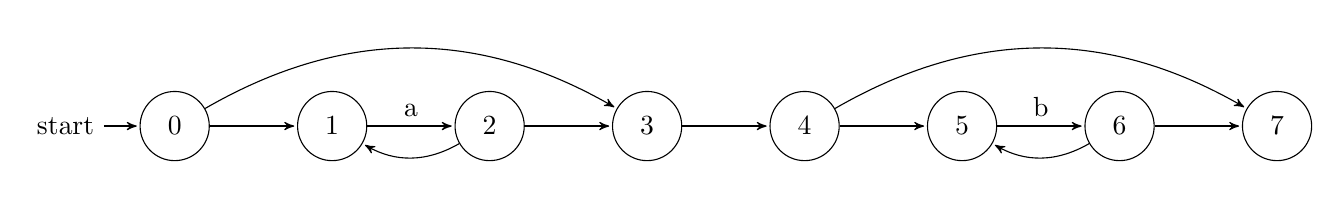
\begin{tikzpicture}[>=stealth',shorten >=1pt,auto,node distance=2cm]
    \node[initial,state]           (0)              {$0$};
    \node[state]                   (1) [right of=0] {$1$};
    \node[state]                   (2) [right of=1] {$2$};
    \node[state]                   (3) [right of=2] {$3$};
    \node[state]                   (4) [right of=3] {$4$};
    \node[state]                   (5) [right of=4] {$5$};
    \node[state]                   (6) [right of=5] {$6$};
    \node[state]                   (7) [right of=6] {$7$};

    \path[->] (0) edge             node {\textepsilon}  (1);
    \path[->] (0) edge [bend left] node {\textepsilon}  (3);
    \path[->] (1) edge             node {a}             (2);
    \path[->] (2) edge             node {\textepsilon}  (3);
    \path[->] (2) edge [bend left] node {\textepsilon}  (1);
    \path[->] (3) edge             node {\textepsilon}  (4);
    \path[->] (4) edge             node {\textepsilon}  (5);
    \path[->] (4) edge [bend left] node {\textepsilon}  (7);
    \path[->] (5) edge             node {b}             (6);
    \path[->] (6) edge             node {\textepsilon}  (7);
    \path[->] (6) edge [bend left] node {\textepsilon}  (5);

  \end{tikzpicture}


\section{Converting an \textepsilon-NFA to an equivalent DFA}
  \begin{itemize}
    \item We can eliminate all \textepsilon-transitions from an \textepsilon-NFA
    by converting it into an equivalent DFA using the subset construction.
    \item Given an \textepsilon-NFA $E = (Q_E, \Sigma, \delta_E, q_E, F_E)$, we
    construct the DFA $D = (Q_D, \Sigma, \delta_D, q_D, F_D)$ as follows:
      \begin{itemize}
        \item $Q_D = P(Q_E)$.
        \item $\delta_D$ is computed all $a$ in $\Sigma$ and $S$ in $P(Q_E)$ as
        follows: \\ Let $S = \{p_1, p_2, \ldots, p_k\}$ and let
        $\{r_1,r_2,\ldots,r_m\}$ be the union of $\delta_E(p_i, a)$ for $i = 1,
        2, \ldots, k$. \\ Then, $\delta_D(S,a) =
        \text{ECLOSE}(\{r_1,r_2,\ldots,r_m\})$.
        \item $q_D = \text{ECLOSE}(q_E)$.
        \item $F_D = \{ \, S | \, S \, \text{is in} \, Q_D \, \text{and} \, S \,
        \text{contains a state in} \, F_E \, \}$.
      \end{itemize}
    \item As with the subset construction, we can prove by induction that
    $L(D) = L(E)$.
  \end{itemize}

  \subsection*{Notes from Class}
    $Q$ represents a set of \textepsilon-transitions. Using the diagram from the
    last section ECLOSE$(Q)$ is $\{0, 1, 3, 4, 5, 7\}$.\\
    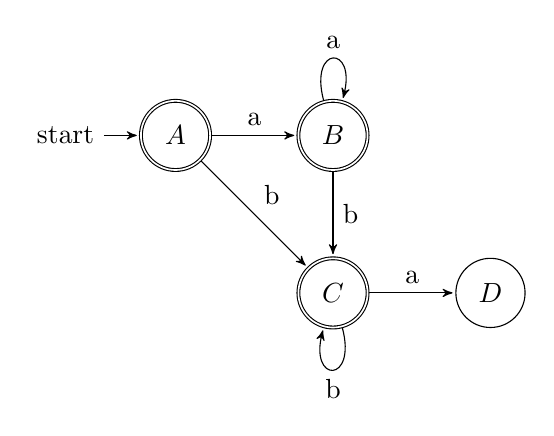
\begin{tikzpicture}[>=stealth',shorten >=1pt,auto,node distance=2cm]
    \node[initial,state,accepting]           (A)              {$A$};
    \node[state,accepting]                   (B) [right of=A] {$B$};
    \node[state,accepting]                   (C) [below of=B] {$C$};
    \node[state]                   (D) [right of=C] {$D$};

    \path[->] (A) edge             node {a}  (B);
    \path[->] (B) edge             node {b}  (C);
    \path[->] (A) edge             node {b}  (C);
    \path[->] (C) edge             node {a}  (D);
    \path[->] (B) edge [loop above] node {a} (B);
    \path[->] (C) edge [loop below] node {b} (C);

  \end{tikzpicture}



\section{Practice Problems}
  \begin{enumerate}
    \item Do the two regular expressions $(a + b)^*$ and $(a^*b^*)^*$ denote the
    same language?
    \item Write a Kleene regular expression for all strings of 0's and 1's with
    an even number of 0's and an even number of 1's.
    \item Let $L$ be the language $\{ \, \texttt{abxba} | \texttt{x} \text{is
    any string of \texttt{a}'s,\texttt{b}'s, and \texttt{c}'s not containing
    \texttt{ba}} \}$. This language models comments in the programming language
    C.
      \begin{enumerate}
        \item Construct a regular expression for $L$.
        \item Show how your regular expression defines the string
              \texttt{abcbaba}.
      \end{enumerate}
    \item Write a Kleene regular expression for all strings of a's and b's that
    begin and end with an a.
    \item Write a Posix regular expression that matches all English words ending
    in dous.
    \item Write a Posix regular expression that matches all English words with
    five vowels a,e,i,o,u in order. (The vowels do not have to be next to one
    another.)
    \item HMU Exercise 2.5.1.
  \end{enumerate}

\section{References}
  \begin{itemize}
    \item HMU: Ch. 2, Sects. 3.1, 3.3.1
    \item \verb|http://en.wikipedia.org/wiki/Regular_expression|
  \end{itemize}

\end{document}
